\documentclass{beamer}
\bibliographystyle{amsalpha}
\usepackage{cite}
\usepackage[normalem]{ulem}
\usepackage{fancybox}
\usepackage{enumitem}
\setitemize{label=\usebeamerfont*{itemize item}
\usebeamercolor[fg]{itemize item}
  \usebeamertemplate{itemize item}}
\setbeamertemplate{footline}[frame number]{}
\setbeamertemplate{navigation symbols}{}
\graphicspath{{figures/}}

\title{The Heterogeneous Multiscale Method}
\subtitle{Combining Molecular Dynamics with Kinetic Theory}
\author[Price and Shohet]{Jake Price and Gil Shohet}
\institute[CPSSW]{Computational Physics Student Summer Workshop}
\date{August 5, 2015}

\begin{document}
	
	\begin{frame}
		\titlepage
	\end{frame}
	
	\section{Heterogeneous Multiscale Method (HMM)}
	\subsection{Overview}
	\begin{frame}{What is the Heterogeneous Multiscale Method (HMM)?}
		\begin{itemize}
		\item Most problems can be viewed on multiple scales\vspace{1em}
		\item HMM is a \textbf{top-down} strategy for creating a \textbf{hybrid method} that uses the microscale model to increase the accuracy of the macroscale model
		\end{itemize}
		
		\begin{center}
			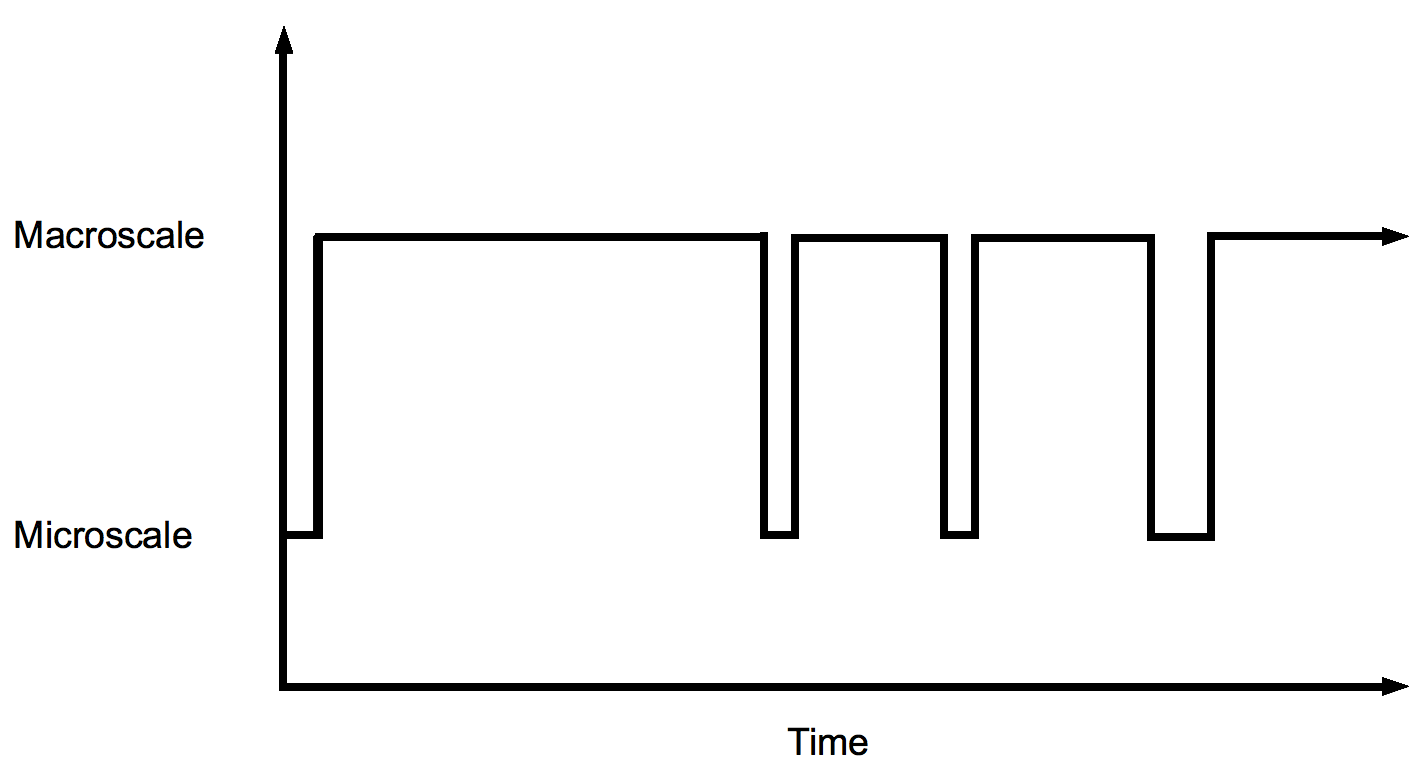
\includegraphics[height = 0.5\textheight]{scheme.png}
			\end{center}
	\end{frame}
	
	\begin{frame}{HMM Structure}
		\begin{itemize}
			\item  A \emph{compression} operator, $Q$, maps information from the microscale state to the macroscale
			\item  A \emph{reconstruction} operator, $R$, reconstructs the microscale model using the macroscale state
		\end{itemize}
		\begin{center}
			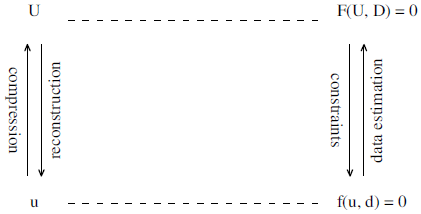
\includegraphics[width=0.7\textwidth]{framework.png}
			\\\tiny HMM Framework (Weinan E et al, 2006)
		\end{center}
	\end{frame}
	
	\begin{frame}{Types of Problems}
		\begin{enumerate}[leftmargin=1.75cm]
			\item[\textbf{Type A:}] Microscopic model is only required near isolated defects or singularities in the domain
			\vspace{2em}
			\item[\textbf{Type B:}] A nearly closed macroscale model exists but is not sufficiently explicit. The microscale model closes the system and provides missing information
		\end{enumerate}
	\end{frame}
	
%	\subsection{Examples}
%	\begin{frame}[t]{Type A Example: Dealing with isolated defects}
%		\begin{itemize}
%			\item  Constitutive relations to compute flux in cells without defects\vspace{1em}
%			\item  Use MD to compute flux in cells that contain defects
%		\end{itemize}
%		\begin{center}
%			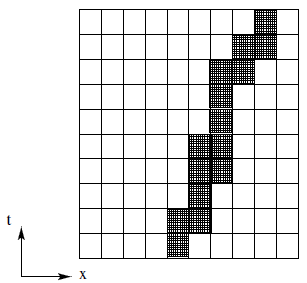
\includegraphics[width=0.5\textwidth]{typeA.png}
%			\\\tiny Movement of defect over time (MD performed in black boxes). (Weinan E et al, 2006)
%		\end{center}
%	\end{frame}
%	
%	\begin{frame}[t]{Type B Example: Large-scale MD gas dynamics}
%		\begin{itemize}
%			\item  Finite volume solver on the macroscale\vspace{1em}
%			\item  Constrained MD on cell boundaries to compute flux
%		\end{itemize}
%		\begin{center}
%			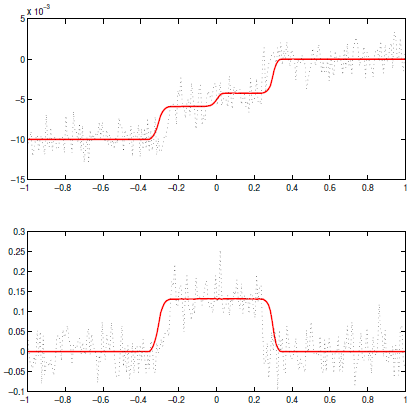
\includegraphics[height=0.65\textheight]{typeB.png}
%			\\\tiny Computed strain (top) and velocity (bottom) compared with full MD simulation. (Weinan E et al, 2006)
%		\end{center}
%	\end{frame}
	
	\section{HMM for Plasma Modeling}
	\subsection{Problem Statement}
	\begin{frame}{Our Goal}
		\begin{itemize}
			\item  Develop a proof-of-concept computational framework to model plasmas using HMM\vspace{1em}
			\begin{itemize}
				\item  We are not trying to model a specific problem\vspace{1em}				\item  We are trying to develop the framework to solve problems using this combination of models\vspace{1em}
			\end{itemize}
			\item  Macroscopic model: Kinetic theory using the BGK approximation of the Boltzmann equation (BGK)\vspace{1em}
			\item  Microscopic model: Molecular dynamics (MD)
		\end{itemize}
	\end{frame}
	
	\begin{frame}{Problem Statement}
		\begin{itemize}
			\item  Ions live in a 2D periodic domain and are initialized with a distribution that is $x$-dependent, but uniform in $y$
			\vspace{0.5em}
			\begin{itemize}
				\item Use data from the 2D-2V MD microscale to increase the accuracy of a 1D-2V BGK macroscale simulation
			\end{itemize}
			\vspace{0.5em}
			\item  The mathematical framework is built up from first principles and designed to be as general as possible
			\vspace{0.5em}
			\item  \emph{Type B} problem: we are using the MD to close our macroscale kinetic model
		\end{itemize}
	\end{frame}
	
	\subsection{Model Formulation}
	\begin{frame}[t]{Microscale MD Model}
		\vspace{1em}
		\begin{itemize}
			\begin{columns}
				\begin{column}{0.9\textwidth}
					\item  2D-2V molecular dynamics with periodic boundary conditions
				\end{column}
				\begin{column}{0.0\textwidth}\end{column}
			\end{columns}
			\vspace{-1.5em}
			\begin{columns}
				\begin{column}{0.5\textwidth}
					\item  Solving a system of simple ODEs:
					\begin{align*}
					\dot{\boldsymbol{x}} &= \boldsymbol{v}	&	\dot{\boldsymbol{v}} &= \frac{\boldsymbol{F}}{m}
					\end{align*}
					\item  Particles interact through the Yukawa potential
					\vspace{0.5em}
					\item  Nearest neighbor lists with cutoff radius for $O(N)$ performance
				\end{column}
				\begin{column}{0.4\textwidth}
					\vspace{1em}
					\begin{center}
						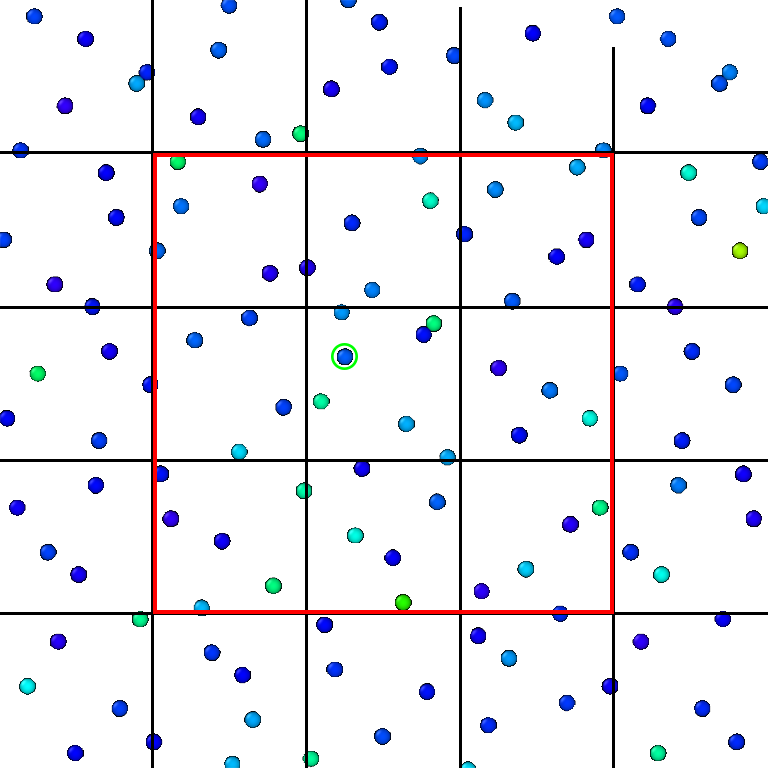
\includegraphics[height=0.5\textheight]{MD_diagram.png}
						\\\tiny MD snapshot with nearest neighbor cells
					\end{center}
				\end{column}
			\end{columns}
		\end{itemize}
	\end{frame}
	
	\begin{frame}{MD Implementation}
		\begin{itemize}
			\item  Velocity Verlet time evolution:\vspace{-0.2em}
			\small\begin{align*}
			v\left(t+\frac{\Delta t}{2}\right) &= v(t) + \frac{\Delta t}{2}\frac{F(t)}{m} \\
			x(t+\Delta t) &= x(t) + \Delta t\:v\left(t+\frac{\Delta t}{2}\right) \\
			v(t+\Delta t) &= v\left(t+\frac{\Delta t}{2}\right) + \frac{\Delta t}{2}\frac{F(t+\Delta t)}{m}
			\end{align*}\normalsize
			\item  Yukawa potential for particles $i$, $j$:\vspace{-0.2em}
			\small\begin{align*}
			V_{ij} &= \frac{Z_iZ_je^2}{4\pi\varepsilon_0r_{ij}}e^{-\frac{r_{ij}}{\lambda}} \\
			F_{ij} &= -\frac{\partial V_{ij}}{\partial r_{ij}} = V_{ij}\left(\frac{1}{r_{ij}}+\frac{1}{\lambda}\right)
			\end{align*}\normalsize
			\item  Track energy to ensure total energy is conserved
		\end{itemize}
	\let\thefootnote\relax\footnotetext{\tiny Thank you to Mathieu Marciante for the base MD code.}
	\end{frame}
	
	\begin{frame}{Kinetic Implementation}
		\begin{itemize}
			\item  We use a second order finite volume method to evolve
			\begin{equation*}
				\frac{\partial f}{\partial t}+v_x\frac{\partial f}{\partial x}+\frac{Z e}{m}E(x,t)\frac{\partial f}{\partial v_x}=\frac{f_{eq}-f}{\tau}
			\end{equation*}
			\begin{itemize}
				\item  The LHS includes terms that describe the evolution of $f$ due advection and the presence of an electric field
				\item The RHS approximates collisional processes by a relaxation towards equilibrium with time scale $\tau$
			\end{itemize}
		\end{itemize}
		\begin{center}
			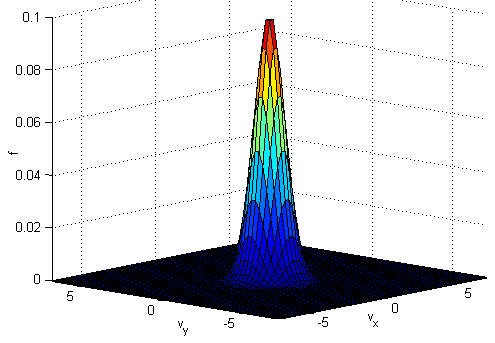
\includegraphics[height=0.3\textheight]{example_f.png}
			\\\tiny $f(\boldsymbol{v})$ at a single $x$ location
		\end{center}
	\let\thefootnote\relax\footnotetext{\tiny Thank you to Jeff Haack for the base KT code.}
	\end{frame}
	
	
	
	\begin{frame}{Comparison of Models}
		\begin{columns}
			\begin{column}{0.55\textwidth}
				\begin{center}\textbf{Molecular Dynamics}\end{center}\vspace{-0.8em}
				\begin{itemize}
					\item  \color{blue}Conserves total energy
					\vspace{0.2em}
					\item  Full particle correlations
					\vspace{0.2em}
					\item  Simulating particle interactions \ovalbox{``exactly''}
					\vspace{0.2em}
					\item  \color{red}Noisy, need ensemble averages
					\vspace{0.2em}
					\item  Tiny time steps
					\vspace{0.2em}
					\item  \ovalbox{Computationally expensive}
				\end{itemize}
			\end{column}
			\begin{column}{0.55\textwidth}
				\begin{center}\textbf{Kinetic Theory}\end{center}\vspace{-0.8em}
				\begin{itemize}
					\item  \color{red}Only conserves kinetic energy
					\vspace{0.2em}
					\item  No knowledge of correlations
					\vspace{0.2em}
					\item  Simulating particle interactions in \ovalbox{average sense}
					\vspace{0.2em}
					\item  \color{blue} Calculate bulk properties easily
					\vspace{0.2em}
					\item  Large time steps
					\vspace{0.2em}
					\item  \ovalbox{Computationally inexpensive}
				\end{itemize}
			\end{column}
		\end{columns}
		\begin{center}
			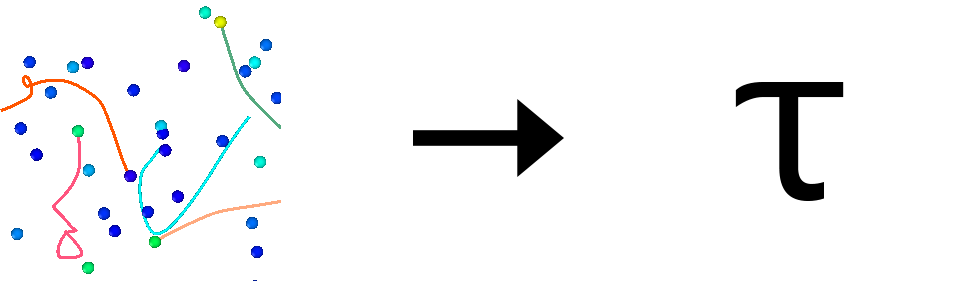
\includegraphics[height=0.3\textheight]{random_walk.png}
		\end{center}
	\end{frame}
	
	\subsection{Connecting the Models}
	\begin{frame}{Connecting the Models with $\tau$}
		\begin{itemize}
		\item BGK attempts to approximate the collisional terms of the Boltzmann equation by relaxing the distribution towards interparticle equilibria with relaxation times $\tau_{kl}$
		\vspace{1em}
		\item Boltzmann also has an $H$ theorem:
		\[H(t)=\int\int  f(\mathbf{r},\mathbf{v},t)\left[\log\left(f(\mathbf{r},\mathbf{v},t)\right)-1\right]\,d\mathbf{r}\,d\mathbf{v}
		\]\item The entropy $-H$ is monotonically increasing
		\vspace{1em}
		\item We choose $\tau$ such that the observed rate of decrease of $H$ in the MD simulation matches the rate of decrease of $H$ in the BGK model
		\end{itemize}
	\end{frame}

	\subsection{Challenges}
	\begin{frame}{Challenges}
		\begin{itemize}
			\item[1. ]  How often do we need to update $\tau$?
			\item[2. ]  How long do we need to run the MD to recover $\tau$?
			\item[3. ]  How do we initialize the MD model from $f$?
			\item[4. ]  How do we return to the BGK model from MD?
		\end{itemize}
		\begin{center}
			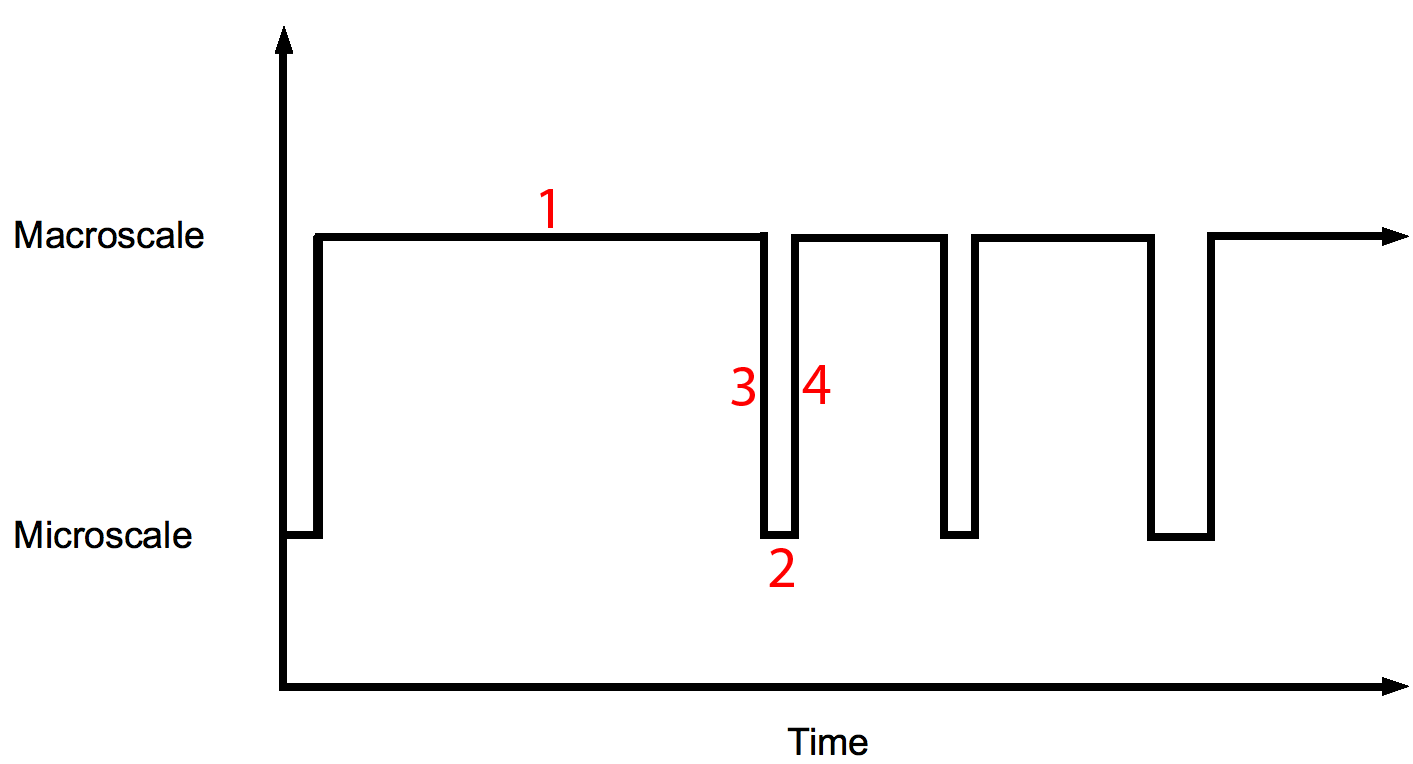
\includegraphics[height=0.55\textheight]{scheme2.png}
		\end{center}
	\end{frame}
	
	\begin{frame}{Reconstruction (How to initialize MD from $f$)}
		\begin{itemize}
		\item $f$ is high dimensional and BGK has no concept of particle correlations
		\vspace{0.5em}
		\item We use a three-step process for initializing MD
		\vspace{0.5em}
		\begin{itemize}
		\item[1. ] Place a set number of particles in $x$ bins to match the density of $f$
		\vspace{0.5em}
		\item[2. ] Use a Langevin thermostat to equilibrate each bin to its proper temperature
		\vspace{0.5em}
		\item[3. ] Once properly correlated, draw new velocities for each particle from the velocity distribution at that $x$ position
		\end{itemize}
		\end{itemize}
	\end{frame}
	
	\begin{frame}{Reconstruction (Equilibration)}
		\begin{itemize}
			\item Uses Langevin dynamics, where $F_i$ is replaced by:
			\begin{equation*}
			F_i = \sum_{j}F_{ij} - m_i\gamma v_i + \sqrt{\frac{2\gamma m_iT}{\Delta t}}\eta
			\end{equation*}
			\item Particles are constrained to their bins with reflective boundary conditions in $x$ to preserve density
		\end{itemize}
		\begin{center}
			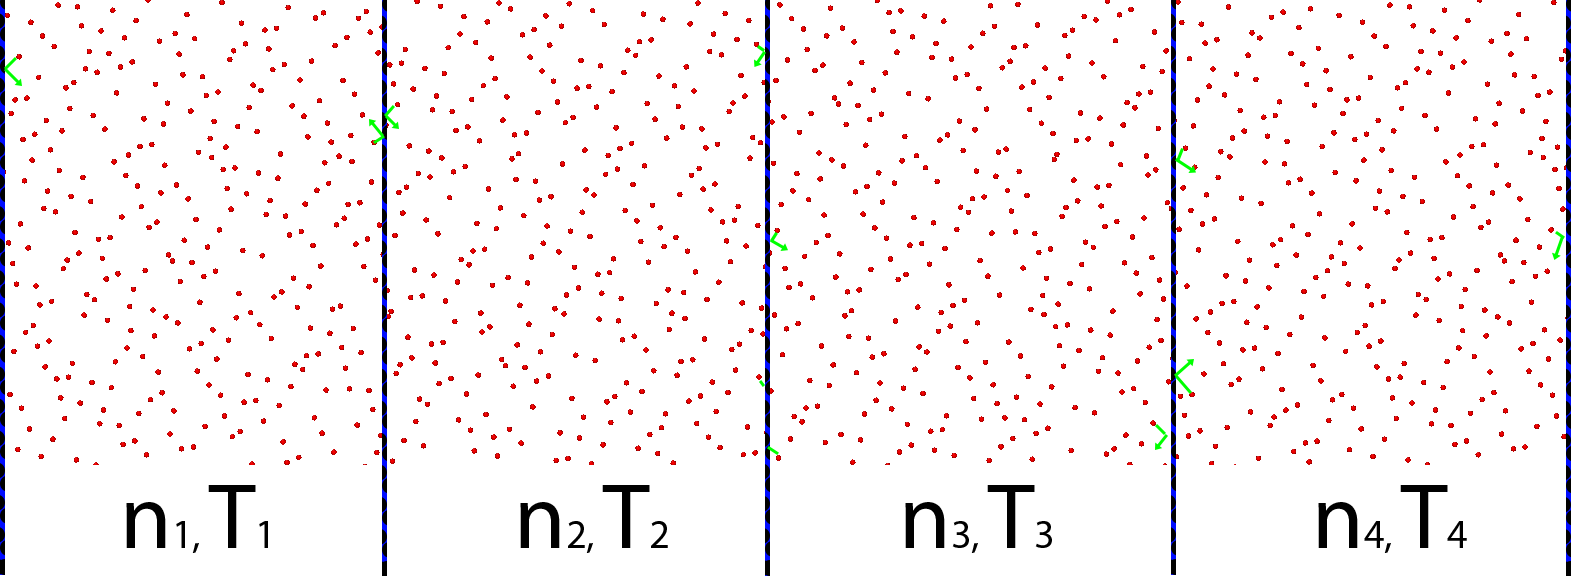
\includegraphics[width=0.9\textwidth]{figures/equilibration.png}
			\\\tiny Scheme for equilibration phase.
		\end{center}
	\end{frame}
	
	\begin{frame}{Reconstruction (Velocity Resample)}
		\begin{itemize}
			\item Assign particle velocities to particles in each bin by sampling the 2D probability distribution function
			\vspace{0.5em}
			\item Our velocity resampling algorithm accurately captures at least the first four moments of the velocity distribution with sufficient particles
			\vspace{0.5em}
		\end{itemize}
		\begin{center}
			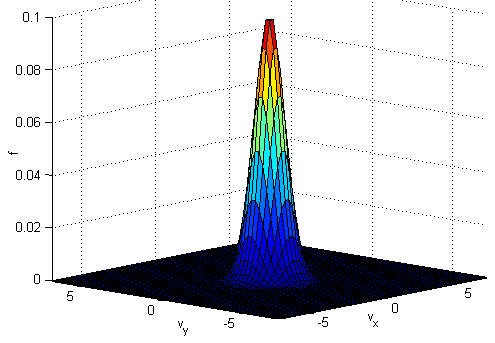
\includegraphics[height=0.4\textheight]{example_f.png}
			\\\tiny Distribution function
		\end{center}
	\end{frame}
	
%	\begin{frame}{Compression (How to go back to BGK from MD)}
%		\begin{itemize}
%		\item We have two options when returning to BGK from MD:
%		\vspace{0.5em}
%		\begin{itemize}
%		\item $f$ is defined as $E[\sum_{i}\delta(\mathbf{r}-\mathbf{r}_i)\delta(\mathbf{v}-\mathbf{v}_i)]$
%		\vspace{0.5em}
%		\begin{itemize}
%		\item When we compute $\tau_{kl}$ using time averages, we can also compute this expected value and reinitialize $f$ at the end time of MD\vspace{0.5em}
%		\end{itemize}
%		\item We can ``pause'' the kinetic distribution, use MD to compute new $\tau_{kl}$ values, and then ``restart'' the BGK simulation where we left off\vspace{0.5em}
%		\end{itemize}
%		\item The first option is more accurate, but is subject to additional statistical noise that the second option avoids
%		\end{itemize}
%	\end{frame}
	
%	\subsection{Results}
%	\begin{frame}{Where are we now?}
%		\begin{itemize}
%		\item 
%		\end{itemize}
%	\end{frame}
	
	\subsection{Preliminary Results}
	\begin{frame}{Preliminary Results}
		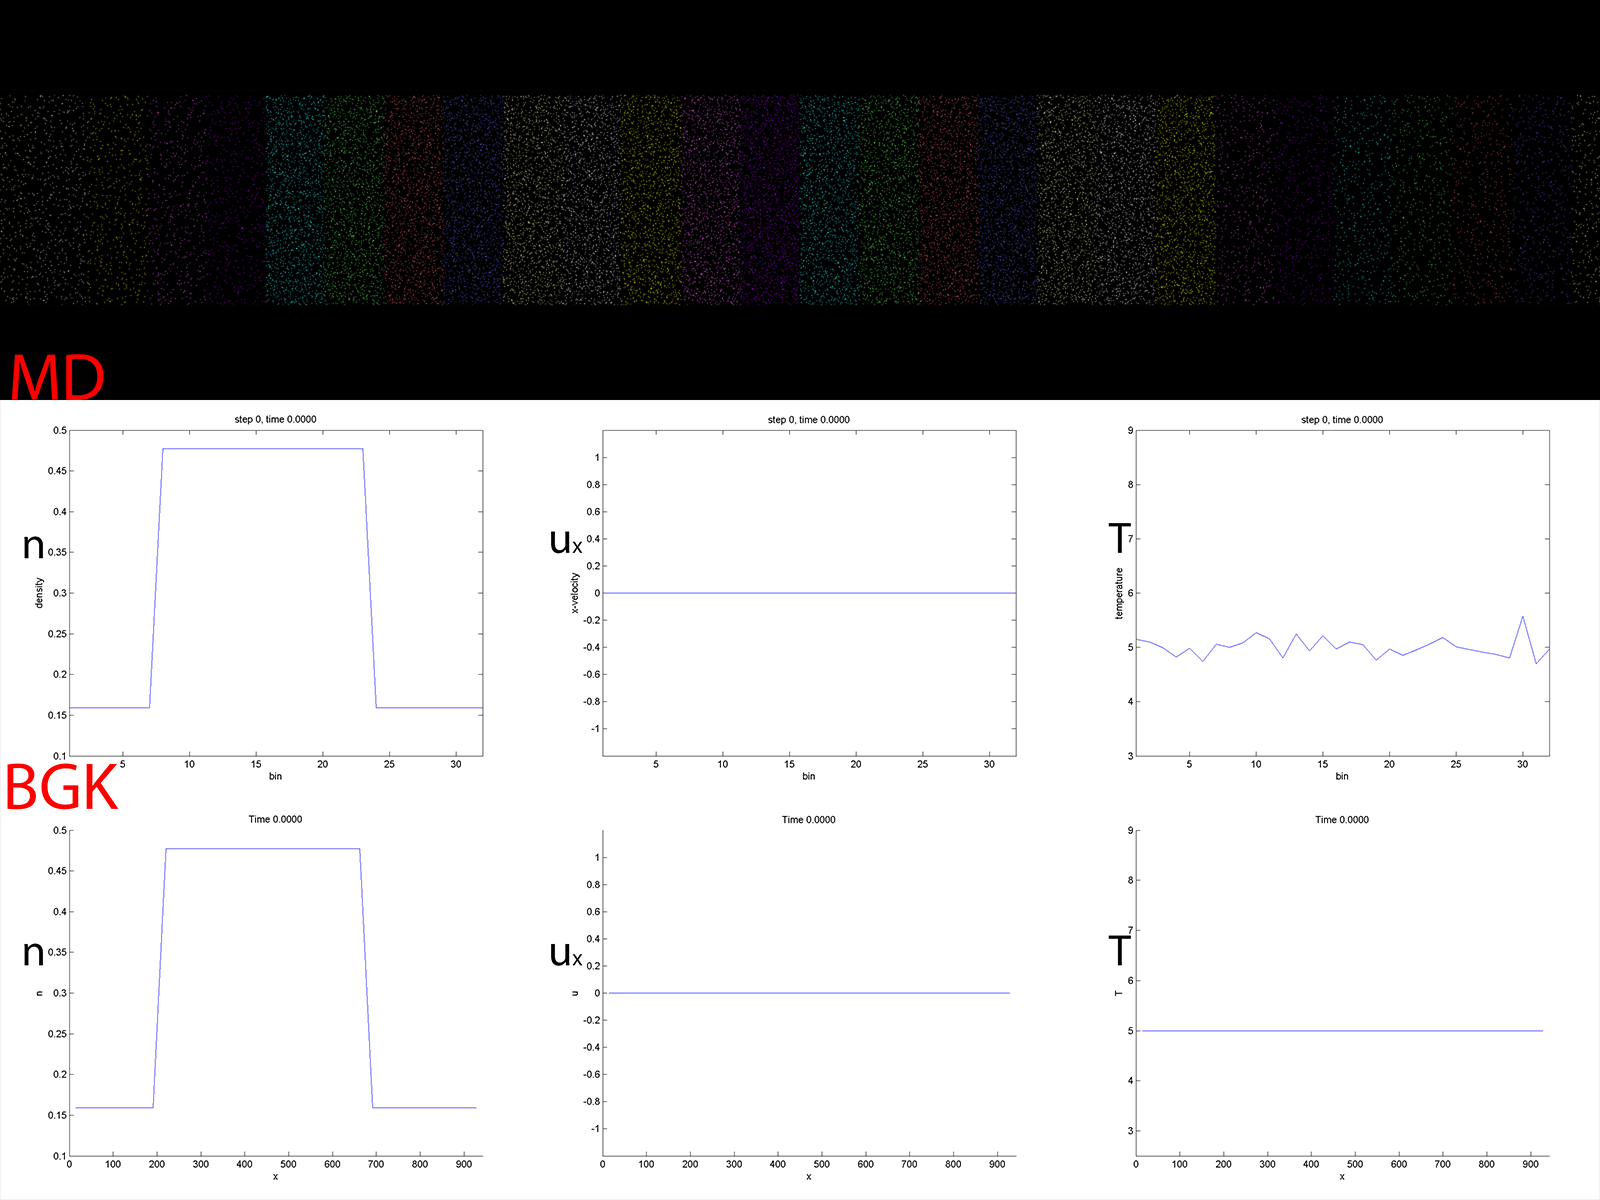
\includegraphics[width=1.0\textwidth]{BGK_MD_movie0000.png}
	\end{frame}
	
	\section{Future Work}
	\begin{frame}{Future Work}
		\begin{itemize}
			\item Implement connection between the KT and MD models and compare results to full MD simulation
			\vspace{0.5em}
			\item Consider alternate ways to compute $\tau$
			\vspace{0.5em}
			\item Implement the model outside Matlab to solve larger problems
			\vspace{0.5em}
			\item Implement in full three dimensions in both regimes
			\vspace{0.5em}
			\item Test model with multi-species scenarios
		\end{itemize}
	\end{frame}

	\section{Summary}
	\begin{frame}{Summary}
		\begin{itemize}
			\item HMM provides a framework to provide hybrid multiphysics simulations that combine the accuracy of the microscale with the efficiency of the macroscale
			\vspace{1em}
			\item Extra attention must be paid to the connection between the two models (compression and reconstruction)
			\vspace{1em}
			\item We have the theoretical framework to model plasmas using kinetic theory and molecular dynamics
		\end{itemize}
	\end{frame}
	
	\section{Acknowledgements}
	\begin{frame}{Acknowledgements}
		We would like to extend our thanks to the following individuals and organizations:\vspace{1em}
		\begin{itemize}
		\item The Los Alamos National Lab Computational Physics Student Summer Workshop for providing a stimulating work environment, and funding our summer research\vspace{1em}
		\item Jeff Haack and Mathieu Marciante for providing the separate BGK and MD codes we used as a starting point\vspace{1em}
		\item Jeff Haack and Michael Murillo for many helpful conversations and overlong meetings
		\end{itemize}
	\end{frame}
	
	\section{References}
	\begin{frame}[allowframebreaks]{References}
	\nocite{weinan2007heterogeneous,weinan2011principles,klimontovich1983kinetic,ren2005heterogeneous,franklin2000boltzmann,hadjiconstantinou1997heterogeneous,flekkoy2000hybrid,nie2004continuum,li1999nearly}
		\bibliography{../../FinalPaper/HMM_bib}
	\end{frame}
	
\end{document}